
\begin{frame}

\section{Introduction}
\frametitle{Introduction}

What is Secure Multi-Party Computation?

- Joint computation of a function
- Secret inputs
- Only final result is revealed

Examples:

- Millionaire's problem
- Secret Santa
- Electronic voting
- Auctions
- Machine learning

\end{frame}




\begin{frame}

\frametitle{MPC Basics}

- Lagrange Interpolation
	- Set of  $t+1$ points uniquely identify a polynomial of degree $\leq t$
- Shamir's Secret Sharing
	- $(t, m)$-threshold secret sharing scheme based on Lagrange Interpolation
	- $\geq$ $t+1$ shares to reconstruct the secret $S$
	- Choose random polynomial $f(x)$ of degree $t$ where $f(0) = S$
	- Share $s_i = f(i)$, for $i \in [1,m]$ 
- Secure Multi-Party Computation
	- $m$ parties jointly compute a function $f(S_{1},S_{2},\dots,S_{m})$, from their secret inputs
	- Party $i$ secret shares its private input $S_{i}$ with the others
	- Interactive protocol to reconstruct a polynomial $g(x)$, where $g(0)=f(S_1, S_2, \dots, S_m)$

\end{frame}




\begin{frame}

\frametitle{Problem Description}

MPyC:

- Python framework for MPC developed at TU/e
- No service discovery yet
- Target users of different level of expertise 
	- Casual
	- Power
	- Enterprise
- MPC is Peer-to-Peer
- Local networks are tricky
	- Limited supply of IPv4 addresses
	- Slow adoption of IPv6
	- Network Address Translation (NAT)

\end{frame}




\begin{frame}

\frametitle{Research Questions}

*How can MPyC be extended to enable casual users, power users and enterprises with limited prior knowledge of each other to discover each other and perform a secure multiparty
computation under diverse networking conditions?*

- deployment strategies?
- identity?
- first contact?
- connectivity?
	- security?
	- privacy?
	- performance?




\end{frame}




\begin{frame}

\frametitle{Preparation Phase Scope}

- Technical Survey
- Extensible Evaluation Environment ($E^3$) - network of host machines for MPC
	- Simple
	- Extensible
	- Cross region
	- Cross platform
	- Automated
	- Reproducible
	- Disposable
- Implementation Phase Planning

\end{frame}




\begin{frame}

\section{Technical Survey}
\frametitle{Technical Survey}

- Deployment tools
- Connectivity approaches

\end{frame}




\begin{frame}

\frametitle{Infrastructure as Code (IaC)}

Tools:

- Provisioning - Terraform, CloudFormation
- Deployment - Ansible, Puppet, Chef

Specification: 

- Imperative - describes the steps to execute
- Declarative - describes the desired state

Operating Systems:

- Most Linux distributions are imperatively managed
- NixOS 
	- Declarative
	- Deployment tools: NixOps, Colmena, morph, deploy-rs 

\end{frame}




\begin{frame}

\frametitle{Virtual Private Networks (VPNs)}

- Centralized VPNs - OpenVPN, IPSec
	- Emulate a real network
	- Transparent to the other programs on the host
	- Single point of failure
	- Can be bottlenecked
- Mesh VPNs - Tailscale, Nebula, Tinc
	- Peer-to-Peer traffic
	- Discovery can happen via a public service or from a known peer 

\end{frame}




\begin{frame}

\frametitle{Network Address Translation (NAT)}

\begin{tabular}{cl}  
 \begin{tabular}{c}
 
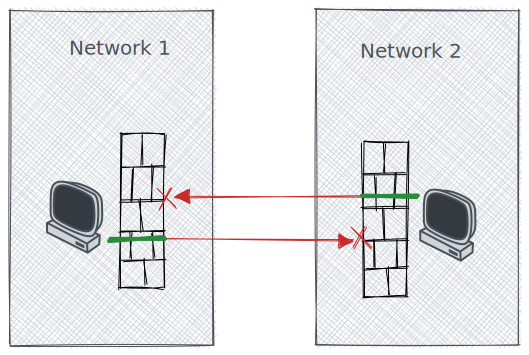
\includegraphics[scale=0.33]{figures/nat-intro.png}
 \end{tabular}
 
& \begin{tabular}{l}

 \parbox{0.5\linewidth}{
 
- Parties behind a NAT device (usually their router)
	- Can initiate a connection to a public endpoint
	- Cannot be discovered from the outside
	- Neither party can initiate the connection to the other

}

 \end{tabular}
\end{tabular} 
\end{frame}


\begin{frame}

\frametitle{NAT Traversal}

\begin{tabular}{cl}  
 \begin{tabular}{c}
 
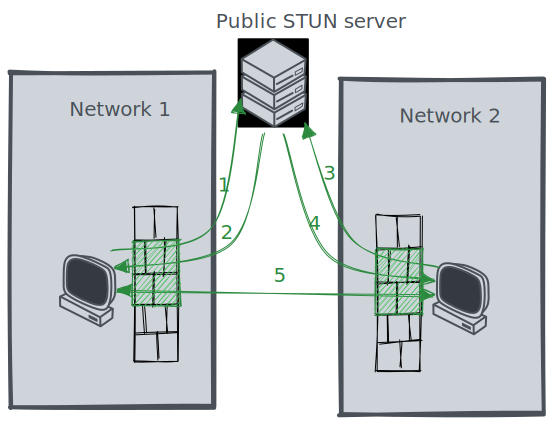
\includegraphics[scale=0.33]{figures/nat-traversal.png}
 \end{tabular}
 
& \begin{tabular}{l}

 \parbox{0.5\linewidth}{

- Session Traversal Utilities for NAT (STUN)
	- Parties connect to a public STUN server (can be another party)
	- The server reports the IPs it "sees" the parties at
	- User Datagram Protocol (UDP) hole punching
		- Reverse channel for the STUN server to talk back to a party
		- Appropriated by the other parties for their own traffic

}

 \end{tabular}
\end{tabular} 
\end{frame}


\begin{frame}

\frametitle{Other approaches}

- Decentralized identifiers (DIDs) and DIDComm
    - Lack of sessions
    - Inefficient for MPC
- The Onion Router
    - Privacy
    - Onion services
- Peer-to-peer applications
    - Bit Torrents
    - Ethereum
    - IPFS

\end{frame}


\begin{frame}

\section{Reference Implementation}
\frametitle{Reference Implementation}

- DigitalOcean - cloud provider
- RaspberryPi - ARM based Single Board Computer (SBC)
- NixOS - declarative Linux distribution
- Terraform - declarative provisioning
- Colmena - declarative NixOS deployment
- Tailscale - mesh VPN as a Service
- prsync - sync directories to multiple hosts over ssh 
- pssh - execute commands on multiple hosts in parallel over ssh

\end{frame}





\begin{frame}

\frametitle{Nix - Basic flake.nix}

```nix
{
  inputs = {
    nixpkgs.url = "github:nixos/nixpkgs/nixos-unstable";
  };

  outputs = inputs@{ self, nixpkgs, ... }:
    let
      pkgs = import nixpkgs {
        system = "x86_64-linux";
      };
    in
    {
		myHello = pkgs.hello;
	};
}
```

\end{frame}





\begin{frame}

\frametitle{Nix - flake.lock}

```nix
{
  "nodes": {
    "nixpkgs": {
      "locked": {
        "lastModified": 1666377499,
        "narHash": "sha256-dZZCGvWcxc7oGnUgFVf0UeNHsJ4VhkTM0v5JRe8EwR8=",
        "owner": "nixos",
        "repo": "nixpkgs",
        "rev": "301aada7a64812853f2e2634a530ef5d34505048",
        "type": "github"
      },
      "original": {
        "owner": "nixos",
        "ref": "nixos-unstable",
        "repo": "nixpkgs",
        "type": "github"
      }
    },
    ...
  }
}
```

\end{frame}





\begin{frame}

\frametitle{Nix - Development Shell}

  ```nix

    devShell.x86_64-linux = pkgs.mkShell {
      shellHook = ''
        export PYTHONPATH=./
      '';
      
      nativeBuildInputs = [
        pkgs.curl pkgs.jq
        pkgs.colmena pkgs.pssh
        (pkgs.terraform.withPlugins
          (tp: [
            tp.digitalocean tp.null
            tp.external tp.tailscale
            tp.random
          ]))
        mpyc-demo
      ];
    };

  ```

\end{frame}





\begin{frame}

\frametitle{Nix - MPyC Package}

``` Nix
{ pkgs, dir }:
(pkgs.poetry2nix.mkPoetryEnv {
    python = pkgs.python3;
    projectDir = dir;
    extraPackages = (ps: [(pkgs.python3Packages.buildPythonPackage {
	      name = "mpyc";
          src = dir;
	    })]);
    overrides = pkgs.poetry2nix.overrides.withDefaults (
      self: super: {
        gmpy2 = pkgs.python3Packages.gmpy2;
      }
    );
  })
```

\end{frame}





\begin{frame}

\frametitle{Nix - DigitalOcean Image (1)}

```nix
## flake.nix
{
  inputs = {
    nixpkgs.url = "github:nixos/nixpkgs/nixos-unstable";
  };
  outputs = inputs@{ self, nixpkgs, ... }:
    let
      mpyc-demo = (import ./nix/mpyc-demo.nix { inherit pkgs; dir = ./.; });
      pkgs = import nixpkgs {
        system = "x86_64-linux";
      };
      digitalOceanConfig = import ./nix/digitalocean/image.nix {
        inherit pkgs;
        extraPackages = [ mpyc-demo ];
      };
    in
    {
		packages.digitalOceanImage = (pkgs.nixos digitalOceanConfig).digitalOceanImage;
	};
}
```

\end{frame}





\begin{frame}
\frametitle{Nix - DigitalOCean Image (2)}

```nix
## nix/digitalocean/image.nix
{ pkgs, extraPackages ? [ ], ... }:
{
  imports = [ "${pkgs.path}/nixos/modules/virtualisation/digital-ocean-image.nix" ];
  system.stateVersion = "22.11";
  environment.systemPackages = with pkgs; [
    jq
  ] ++ extraPackages;
  
  services.tailscale.enable = true;

  networking.firewall = {
    enable = true;
    checkReversePath = "loose";
    trustedInterfaces = [ "tailscale0" ];
  };
}
```

\end{frame}





\begin{frame}

\frametitle{Nix - RaspberryPi Image}

```nix
let
  mpyc-demo = (import ./nix/mpyc-demo.nix { inherit pkgs; dir = ./.; });

  pkgs = import nixpkgs {
	system = "aarch64-linux";
  };
in
{
	packages.raspberryPi4Image = (pkgs.nixos ({ config, ... }: {
		system.stateVersion = "22.11";
		imports = [
		  ("${pkgs.path}/nixos/modules/installer/sd-card/sd-image-aarch64-installer.nix")
		];
		
		environment.systemPackages = [
			mpyc-demo
		];
	})).sdImage;
};
```

\end{frame}





\begin{frame}

\frametitle{Terraform - Image Import}

```terraform
resource "digitalocean_spaces_bucket_object" "nixos-image" {
  region = digitalocean_spaces_bucket.tf-state.region
  bucket = digitalocean_spaces_bucket.tf-state.name
  key    = basename(var.nixos-image-path)
  source = var.nixos-image-path
  acl    = "public-read"
  etag   = filemd5(var.nixos-image-path)
}

resource "digitalocean_custom_image" "nixos-image" {
  name    = "nixos-22.11"
  url     = "https://${digitalocean_spaces_bucket.tf-state.bucket_domain_name}/${digitalocean_spaces_bucket_object.nixos-image.key}"
  regions = local.all_regions
  tags    = ["nixos"]

  lifecycle {
    replace_triggered_by = [
      digitalocean_spaces_bucket_object.nixos-image
    ]
  }
}
```

\end{frame}





\begin{frame}

\frametitle{Terraform - Hostname Generation}

```terraform
locals {
  node_definitions = var.DESTROY_NODES != "" ? [] : [
    { region = "ams3", num = 3 },
    { region = "sfo3", num = 1 },
    { region = "nyc3", num = 1 },
    { region = "sgp1", num = 1 },
  ]
  nodes_expanded = flatten([
    for node in local.node_definitions : [
      for i in range(node.num) :
      merge(node, {
        name = "mpyc-demo--${node.region}-${i}"
      })
    ]
  ])
  nodes = {
    for node in local.nodes_expanded :
    node.name => merge(node, {
      hostname = "${node.name}-${random_id.mpyc-node-hostname[node.name].hex}"
    })
  }
}
```

\end{frame}





\begin{frame}

\frametitle{Terraform - DigitalOcean Droplets}

```terraform
resource "digitalocean_droplet" "mpyc-node" {
  for_each = local.nodes

  image    = digitalocean_custom_image.nixos-image.id
  name     = each.value.hostname
  region   = each.value.region
  size     = "s-1vcpu-1gb"
  ssh_keys = [for key in digitalocean_ssh_key.ssh-keys : key.fingerprint]

  provisioner "remote-exec" {
    inline = [
      "mkdir -p /var/keys/",
      "echo ${tailscale_tailnet_key.keys.key} > /var/keys/tailscale",
      "tailscale up --auth-key file:/var/keys/tailscale"
    ]
  }
}

resource "tailscale_tailnet_key" "keys" {
  ...
}
```

\end{frame}





\begin{frame}

\frametitle{Colmena}

``` nix
let
  mpyc-demo = (import ./nix/mpyc-demo.nix { inherit pkgs; dir = ./.; });

  pkgs = import nixpkgs {
	system = "x86_64-linux";
  };

  digitalOceanConfig = import ./nix/digitalocean/image.nix {
	inherit pkgs;
	extraPackages = [ mpyc-demo ];
  };
in
{
  packages.colmena = {
	meta = {
	  nixpkgs = pkgs;
	};
	defaults = digitalOceanConfig;
  } // builtins.fromJSON (builtins.readFile ./hosts.json);
};
```

\end{frame}





\begin{frame}

\frametitle{Colmena - hosts.json}

``` json
## hosts.json
{
  "mpyc-demo--ams3-0-15e53f39": {},
  "mpyc-demo--ams3-1-b4791c55": {},
  "mpyc-demo--ams3-2-7f09fb08": {},
  "mpyc-demo--nyc3-0-7dd0d9f6": {},
  "mpyc-demo--sfo3-0-5bffc60e": {},
  "mpyc-demo--sgp1-0-92700733": {}
}
```

\end{frame}





\begin{frame}

\frametitle{Runtime}

```bash
prsync -h hosts.pssh -zarv -p 4 ./ /root/mpyc
pssh -h hosts.pssh -iv -o ./logs/$t "cd /root/mpyc && ./prun.sh"
```

``` bash
# assemble $args and $MY_PID from the hosts.pssh file
...

if [ $MY_PID = -1 ]
then
    echo Only $i parties are allowed. $HOSTNAME will not participate in this MPC session
else

cmd="python ./demos/secretsanta.py 3 --log-level debug \
    -I ${MY_PID} \
    ${args}"

echo $cmd
$cmd
fi
```

\end{frame}




\begin{frame}

\section{Demo}
\frametitle{Demo}

- Provisioning with Terraform
- Deployment with Colmena
- Running a distributed MPyC program
- Destruction of the infrastructure

\end{frame}



\begin{frame}

\section{Planning}
\frametitle{Planning - connectivity implementations}

- Headscale
- Nebula - IP allocation, Certificate authority, Certificate distribution
- Mesh VPN with alternative identity management
	- MPC based CA
	- Decentralized Identifiers
- DIDComm
	- sessions
	- NAT traversal
- TOR, Ethereum, IPFS
- Carbyne stack

\end{frame}



\begin{frame}

\frametitle{Planning - analysis}

Compare the implementations in terms of:

- Security
- Performance
- Ease of use
- Privacy

\end{frame}


